\chapter{ОЦЕНКА ПАРАМЕТРОВ ОШИБОК В ВИРТУАЛЬНОМ КАНАЛЕ}
\label{chap:CNM}

\section{Вводные замечания}
\label{chap:CNM:Intro}

Интерпретация процесса сжатия видеоданных в распределенных видеокодеках с использованием понятия виртуального канала была рассмотрена в разделе~\ref{chap1}. На качественном уровне была обоснована важность задачи оценки параметров ошибок, возникающих в виртуальном канале. В данном разделе рассматриваются вопросы, связанные с оценкой параметров ошибок межкадрового предсказания на практике. Отметим, что в англоязычной литературе эта задача также иногда называется~\emph{моделированием виртуального канала} (Virtual Dependency Channel Modeling) или~\emph{моделированием корреляционного шума} (Correlation Noise Modeling).

Рассмотрим формирование ошибок межкадрового предсказания в рамках распределенного видеокодирования в спектральной области с использованием концепции Стэнфорд. Обозначим результат предсказания промежуточного кадра на стороне декодера через $\mathbf{F}_a$. Следует отметить, что т.~к. кодек DISCOVER обрабатывает только однокомпонентные видеопоследовательности, здесь и далее будем считать, что $\mathbf{F}_a$ содержит яркостную составляющую. Декодер, аналогично кодеру, выполняет блоковое спектральное преобразование и квантование для пикселей кадра $\mathbf{F}_a$, в результате чего для каждой группы спектральных коэффициентов формируется набор индексов квантов $\hat{\mathbf{q}}^{(b)}=(\hat{q}^{(b)}_1,\hat{q}^{(b)}_2,...,\hat{q}^{(b)}_m)$, где $b$~--~номер группы, $m$~--~число спектральных коэффициентов в группе. Отметим, что кодер, выполнив аналогичные операции, получает набор индексов квантов $\mathbf{q}^{(b)}=(q^{(b)}_1,q^{(b)}_2,...,q^{(b)}_m)$ для оригинального промежуточного кадра~$\mathbf{F}_i$.
Так как результат предсказания является некоторой аппроксимацией промежуточного кадра, $\mathbf{q}^{(b)}$ и $\hat{\mathbf{q}}^{(b)}$ можно рассматривать как выходы зависимых источников. Таким образом, $\hat{\mathbf{q}}^{(b)}$ является дополнительной информацией декодера и ошибка межкадрового предсказания в спектральной области $\mathbf{n}^{(b)}=(n^{(b)}_1,n^{(b)}_2,...,n^{(b)}_m)$ для каждой группы определяется как
\begin{equation*}
\mathbf{n}^{(b)} = \mathbf{q}^{(b)} - \hat{\mathbf{q}}^{(b)}.
\end{equation*}
Наличие различий между квантованными спектральными коэффициентами на стороне кодера и декодера, объясняется в первую очередь несовершенством алгоритмов аппроксимации промежуточного кадра. Отметим также, что так как оригинал кадра доступен только кодеру, декодер не может в явном виде рассчитать~$\mathbf{n}^{(b)}$.

Учитывая вышесказанное, задачу декодера при оценке параметров ошибок межкадрового предсказания можно сформулировать следующим образом: не зная точные значения ошибок~$n^{(b)}_i$, оценить для каждого квантованного спектрального коэффициента~$\hat{q}^{(b)}_i$ набор некоторых характеристик, описывающих шум, возникающий в виртуальном канале при <<передаче>> данного коэффициента. Данные характеристики далее используются декодером для формирования мягкого входа помехоустойчивого декодера в кодеке Слепяна-Вулфа. В рамках приведенной задачи можно выделить следующие подзадачи:
\begin{itemize}
\item аппроксимация шума $\mathbf{n}^{(b)}$ на стороне декодера;
\item определение параметров ошибки для каждого квантованного спектрального коэффициента~$\hat{q}^{(b)}_i$.
\end{itemize}

Рассмотрению этих вопросов и посвящен данный раздел. В подразделе~\ref{chap:CNM:ReferenceAlgo} приводится набор общепринятых допущений об ошибках, возникающих в виртуальном канале, и рассматривается алгоритм оценки параметров ошибок межкадрового предсказания, используемый в кодеке DISCOVER. Указаны основные недостатки данного алгоритма и предложена модифицированный алгоритм, лучше выполняющий учет особенностей ошибок межкадрового предсказания. В подразделе~\ref{chap:CNM:ProposedModel} предложен новый, расширенный набор допущений, на основе которого разработана обобщенная модель виртуального канала, основанная на представлении ошибок как случайного процесса, задаваемого Марковской сетью со скрытыми состояниями. Для этой модели показано, что задачу оценки параметров ошибок можно свести к задаче согласованной маркировки (раскрашивания) вершин некоторого графа, причем решение этой задачи соответствует оценке по методу максимального правдоподобия. Показано, что в рамках введенной модели результат модифицированного алгоритма лучше, чем у базового алгоритма. Основные результаты данного раздела опубликованы в работах~\cite{Icumt2014},~\cite{KES2015},~\cite{Suai2011}.

\section{Существующие методы оценки параметров ошибок межкадрового предсказания для систем распределенного кодирования}
\label{chap:CNM:ReferenceAlgo}

\subsection{Описание общепринятых допущений о виртуальном канале}
\label{chap:CNM:ReferenceAlgo:CommonAssumptions}

В ранних работах по распределенному кодированию источников видеоинформации ошибка межкадрового предсказания рассматривалась как аддитивный случайный стационарный процесс с нулевым математическим ожиданием~\cite{1246773}. Это допущение известно как~\emph{стационарный виртуальный канал}. Термин <<стационарность>> в данном контексте означает, что вероятностные характеристики ошибок не меняются в рамках одной группы спектральных коэффициентов для одного кадра. Одним из существенных преимуществ такой модели шума является простота её реализации на практике. Однако, в силу того, что алгоритмы аппроксимации промежуточных кадров в распределенном видеокодировании основаны на различных методах временной интерполяции/экстраполяции, вероятностные характеристики ошибок межкадрового предсказания на практике могут существенно различаться. Например, интенсивность ошибок в областях на кадрах, где появляются новые объекты или наблюдается сложное движение существующих объектов, существенно превышает интенсивность ошибок в областях с малоподвижным фоном (рисунок~\ref{fig:chap3:RealResidual}). Таким образом, модель, основанная на допущении о стационарном виртуальном канале, плохо подходит для описания ошибок межкадрового предсказания. В связи с этим в современных работах по распределенному видеокодированию рассматриваются модели шума, основанные на допущении о~\emph{нестационарном виртуальном канале}.

\begin{figure}[t]
  \centering
  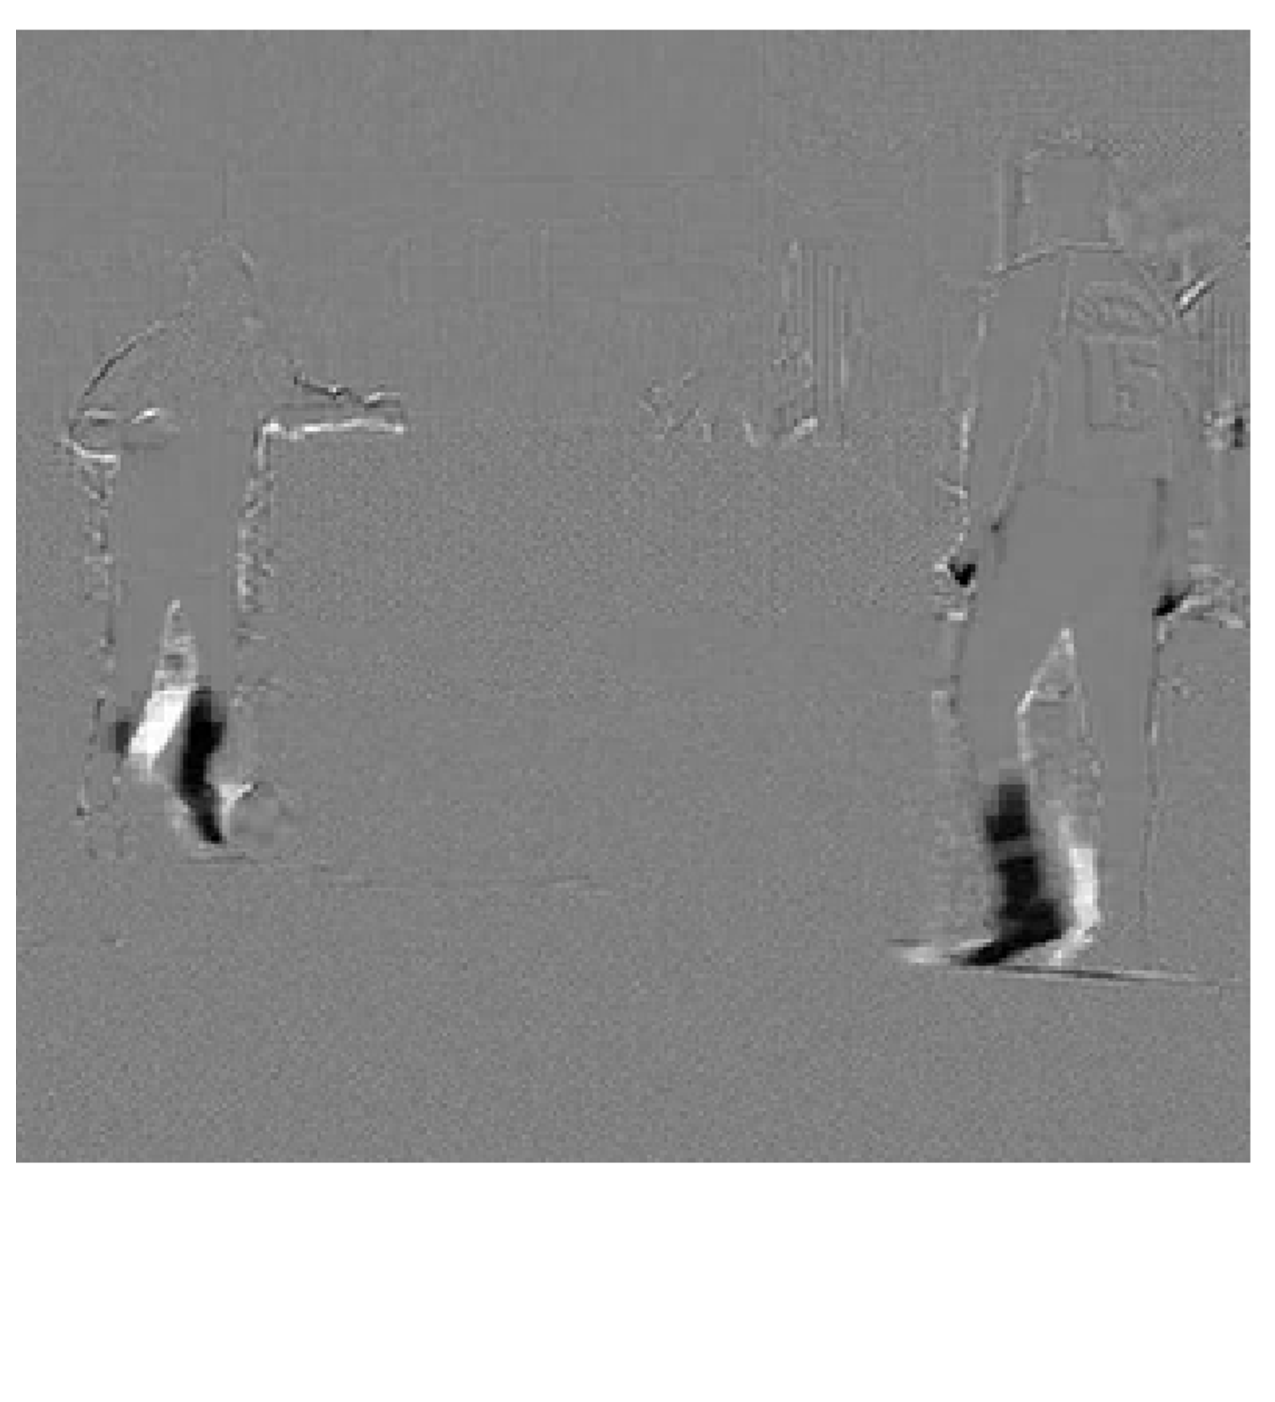
\includegraphics[width=0.8\linewidth]{Chapter3/RealResidual}
  \caption{Пример ошибок межкадрового предсказания для кадра из последовательности SOCCER (значение $128$ соответствует нулевой ошибке)}
  \label{fig:chap3:RealResidual}
\end{figure}

Рассмотрим набор общепринятых допущений о нестационарном виртуальном канале~\cite{borchert2010distributed}.

\begin{assumption}
  Для каждой группы спектральных коэффициентов декодер может выполнить аппроксимацию ошибок~$\hat{\mathbf{n}}^{(b)} = ( \hat{n}^{(b)}_{1}, \hat{n}^{(b)}_{2},\ldots,\hat{n}^{(b)}_{m})$, причем $\hat{n}^{(b)}_{i} = n^{(b)}_{i} + e^{(b)}_{i}$, где $e^{(b)}_{i}$~--~случайное искажение, имеющее некоторый закон распределения с нулевым математическим ожиданием и конечной дисперсией.
  \label{ass:1}
\end{assumption}
Будем называть $\hat{\mathbf{n}}^{(b)}$ \emph{аппроксимацией} ошибки межкадрового предсказания на стороне декодера.
%\begin{assumption}
%  Шум - это последовательность $n^{(b)}_{i}$ одинаково распределенных случайных величин из некоторого вероятностного закона, функцию плотности вероятности которого можно аппроксимировать смесью распределений Лапласа с нулевым математическим ожиданием
%  \begin{equation*}
%  f(x) = \sum\limits_{i=1}^{k} w_i^{(b)} \mathrm{Lap}(x \vert \alpha_i ,0),
%  \label{eq:LMM}
%  \end{equation*}
%  где $w_i^{(b)}$~--~вес соответствующей компоненты смеси, $\mathrm{Lap}(x \vert \alpha_i ,\mu_i)$~--~функция плотности вероятности распределения Лапласа с параметрами $\alpha_i$ (масштаб) и $\mu_i$ (математическое ожидание), задаваемая как
%  \begin{equation*}
%  \mathrm{Lap}(x \vert \alpha_i ,\mu_i) = \frac{\alpha_i}{2} e^{-\alpha_i |x-\mu_i|}.
%  \end{equation*}
%  \label{ass:2}
%\end{assumption}
\begin{assumption}
    Виртуальный канал является каналом с аддитивным нестационарным Лапласовым шумом, т.~е. каждое значение $n^{(b)}_{i}$ является реализацией случайной величины $N^{(b)}_{i}$, имеющей закон распределения Лапласа с нулевым математическим ожиданием:    
    \begin{equation*}
        N^{(b)}_{i} \sim \mathrm{Lap}(x \vert \alpha^{(b)}_{i} ,0),
    \end{equation*}
    где
    \begin{equation*}
        \mathrm{Lap}(x \vert \alpha^{(b)}_i ,\mu^{(b)}_i) = \frac{\alpha^{(b)}_i}{2} e^{-\alpha^{(b)}_i |x-\mu_i|}.
    \end{equation*}
  \label{ass:2}
\end{assumption}

Отметим, что допущение~\ref{ass:2} позволяет рассматривать последовательность ошибок $n^{(b)}_{i}$ как реализацию множества в общем случае зависимых случайных величин, хотя понятие зависимости при этом никак не формализуется. Единственное, что утверждается, это то, что условная функция плотности вероятности для каждой ошибки является Лапласовой.

С учетом приведенных допущений, задача оценки параметров ошибок межкадрового предсказания заключается в оценке для каждого квантованного спектрального коэффициента параметра масштаба распределения Лапласа, описывающего интенсивность искажающего воздействия, <<возникающего>> в виртуальном канале при передаче данного спектрального коэффициента. Для решения данной задачи в модели Discover предлагается эвристический алгоритм, описанный в следующем подразделе.

\subsection{Описание базового алгоритма оценки параметров ошибок межкадрового предсказания}
\label{chap:CNM:ReferenceAlgo:AlgoDescription}

Рассмотрим алгоритм моделирования виртуального канала, разработанный в рамках проекта DISCOVER~\cite{4498429}. Здесь и далее будем придерживаться обозначений, введенных в разделе~\ref{chap:SIG}. 

Процедура оценки параметров ошибок межкадрового предсказания в кодеке DISCOVER представляет собой следующую последовательность действий.

\begin{enumerate}
  \item Расчет аппроксимации ошибки в пространственной области. В базовом алгоритме ошибку аппроксимации в пространственной области предлагается рассчитывать как 
  \begin{equation*}
    \mathbf{R}(\mathbf{p}) = \frac{1}{2} \left[ \mathbf{F}_p(\mathbf{p}-\mathbf{V}(\mathbf{p})) + \mathbf{F}_f(\mathbf{p}_i+\mathbf{V}(\mathbf{p}))\right], \forall \mathbf{p} \in \mathcal{P},
    \label{eq:NoiseEstimation}
  \end{equation*}  
  где $\mathbf{F}_p$, $\mathbf{F}_f$~--~опорные кадры, находящиеся во времени соответственно перед и после промежуточного кадра, $\mathbf{V}(\mathbf{p})$~--~билатеральное векторное поле, полученное в результате процедуры оценки движения (подраздел~\ref{chap:SIG:ReferenceAlgo}), $\mathcal{P}$~--~множество позиций пикселей.
  
  \item Расчет оценки шума $\hat{\mathbf{n}}^{(b)}$. Разностный кадр $\mathbf{R}$ подвергается блоковому дискретному косинусному преобразованию с размером блока $4 \times 4$ пикселя. Затем, по аналогии с обработкой аппроксимирующего кадра $\mathbf{F}_a$, полученные спектральные коэффициенты собираются в группы $\mathbf{n}^{(b)}$ (детальное описание процесса приведено в подразделе~\ref{chap:CNM:Intro}). Делается допущение, что рассчитанные таким образом данные являются аппроксимацией ошибок межкадрового предсказания на стороне декодера.
  
  \item Расчет выборочного среднего для абсолютных значений оцененных ошибок:
  \begin{equation*}
  \forall b \in \{1,2,\ldots, B\}: \hat{\mu}^{(b)} = \frac{1}{m}  \sum\limits_{i=1}^{m} \vert \hat{n}^{(b)}_i \vert.
  \end{equation*}
  
  \item Расчет для каждого оцененного значения шума квадратичного отклонения от выборочного среднего
  \begin{equation*}
  \forall b \in \{1,2,\ldots, B\}, \forall i \in \{1,2,\ldots, m\}: d^{(b)}_i = \left( \vert \hat{n}^{(b)}_i \vert - \hat{\mu}^{(b)} \right)^2.
  \end{equation*}
  
  \item Расчет выборочной дисперсии для абсолютных значений оцененных ошибок:
  \begin{equation*}
  \forall b \in \{1,2,\ldots, B\}: \left(\hat{\sigma}^{(b)}\right)^2 = \frac{1}{m} \sum\limits_{i=1}^{m} d^{(b)}_i.
  \end{equation*}
  
  \item Оценка параметра распределения Лапласа для группы:
  \begin{equation*}
  \forall b \in \{1,2,\ldots, B\}: \hat{\alpha}^{(b)} = \frac{\sqrt{2}}{\hat{\sigma}^{(b)}}
  \end{equation*}
  
  \item\label{algo:DiscoverCNM:FinalEstmation} Оценка параметра распределения Лапласа для каждого коэффициента:
  \begin{equation*}
  \forall b \in \{1,2,\ldots, B\}, \forall i \in \{1,2,\ldots, m\}:
  \hat{\alpha}^{(b)}_i = 
  \begin{cases}
  & \hat{\alpha}^{(b)},\text{ если $d^{(b)}_i \leq \sigma^{(b)}$} \\
  & \frac{\sqrt{2}}{d^{(b)}_i},\text{ иначе}
  \end{cases}.
  \end{equation*}

\end{enumerate}

В дальнейшем будем называть данный алгоритм \emph{базовым алгоритмом} оценки параметров ошибок межкадрового предсказания. Отметим, что в базовом алгоритме нестационарность ошибок в виртуальном канале учитывается  с помощью адаптации оценки параметра распределения Лапласа для каждого спектрального коэффициента с учетом статистики всех коэффициентов в группе.

\subsection{Недостатки базового алгоритма}
\label{chap:CNM:ReferenceAlgo:Troubles}

Рассмотрим пример, в рамках которого продемонстрируем работу базового алгоритма, а также выявим ряд его потенциальных недостатков. Данный пример будет использован в следующем подразделе для демонстрации особенностей предложенной модели шума. Рассмотрим процесс восстановления промежуточного кадра на стороне декодера. Декодер, восстановив пару смежных опорных кадров, выполняет по ним аппроксимацию промежуточного кадра (например, с использованием алгоритма, описанного в подразделе~\ref{chap:SIG:ReferenceAlgo} и рассчитывает оценку ошибки межкадрового предсказания (например, с использованием подхода, описанного в подразделе~\ref{chap:CNM:ReferenceAlgo}). Результат данных операций представлен на рисунке~\ref{fig:chapCNM:ExampleMain}. Также, для того, чтобы продемонстрировать тот факт, что результат оценки ошибки межкадрового предсказания коррелирует с реальной ошибкой, на данном рисунке приведена разность между восстановленным промежуточным кадром на стороне кодера и его аппроксимацией на стороне декодера.

\begin{figure}[htbp]
    \centering
    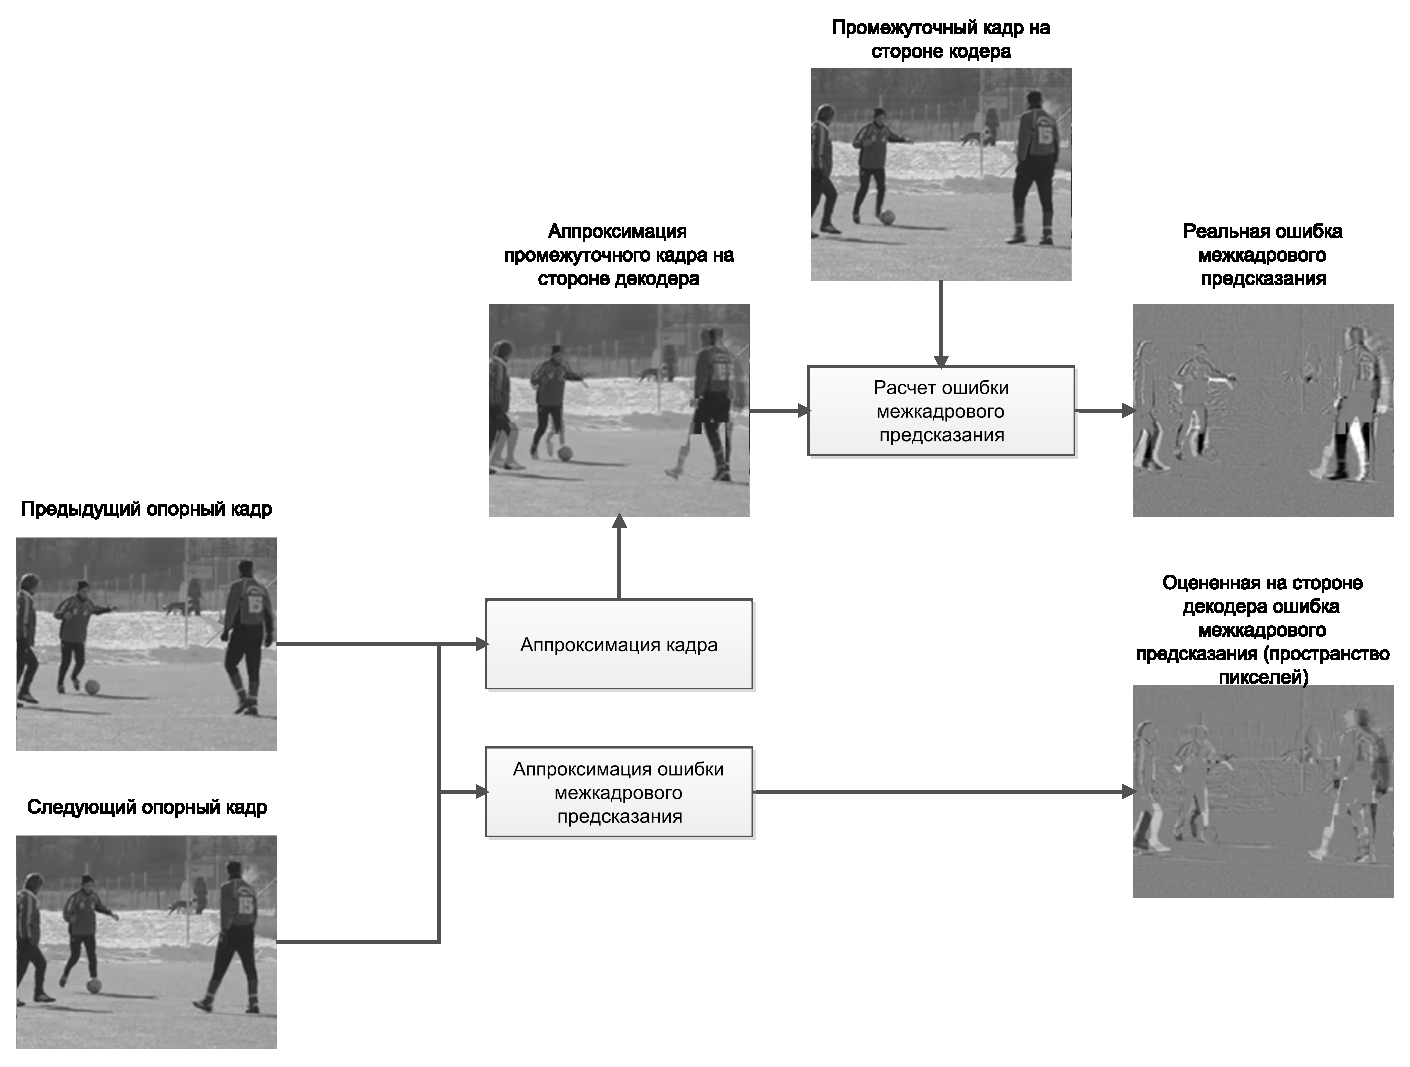
\includegraphics[width=0.85\textwidth]{Chapter3/ExampleMain}
    \caption{Пример оцененной на стороне декодера ошибки межкадрового предсказания в пространстве пикселей}
    \label{fig:chapCNM:ExampleMain}
\end{figure}

Аппроксимация ошибки в спектральной области для старшего коэффициента, рассчитанная по оцененной на стороне декодера ошибке межкадрового предсказания, представлена на рисунке~\ref{fig:chapCNM:ExampleBand}. Видно, что особенность шума, связанная с группировкой ошибок в пространстве пикселей, сохранилась и в спектральной области. Отметим, что т.~к. базовый алгоритм работает только с абсолютными значениями коэффициентов, на рисунке приведены абсолютные величины оцененных ошибок. Для того, чтобы продемонстрировать работу базового алгоритма, рассмотрим процесс оценки параметров ошибок для части спектральных коэффициентов, отмеченных на рисунке~\ref{fig:chapCNM:ExampleBand}. В целях демонстрации будем считать, что в аппроксимации шума для данной группы частот содержатся только эти коэффициенты, т.~е.
\begin{equation}
    \hat{\mathbf{n}}^{(1)} = 
    \left(
    \begin{matrix}
        2 &  1 &   3 &   5 \\
        0 &  0 &   4 &  83 \\
        7 & 24 & 157 & 208 \\
        1 &  1 &  30 & 132
    \end{matrix}
    \right).
    \label{eq:chapCNM:NoseDemo}
\end{equation}

\begin{figure}[htbp]
    \centering
    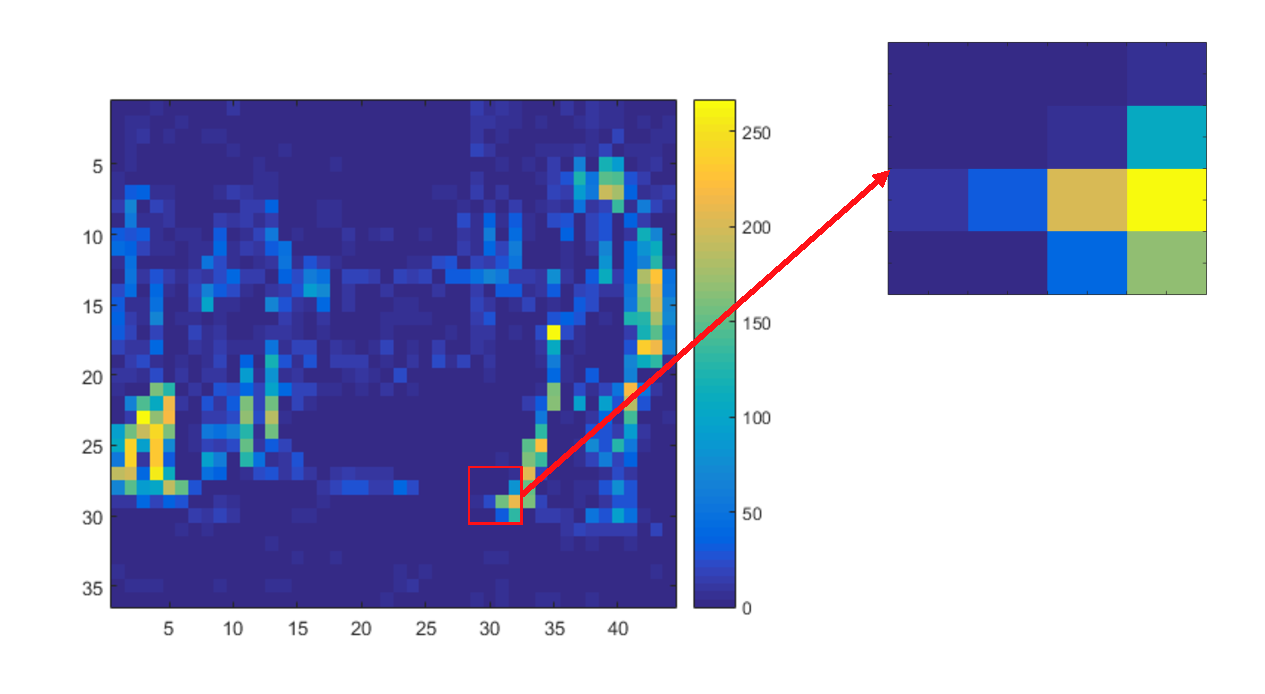
\includegraphics[width=0.8\textwidth]{Chapter3/ExampleBand}
    \caption{Пример аппроксимации ошибок межкадрового предсказания в спектральной области (коэффициент DC).}
    \label{fig:chapCNM:ExampleBand}
\end{figure}

Приведем шаги алгоритма для данных значений. Т.~к. шаги 1 и 2 связаны с получением аппроксимации шума, начнем пример с шага 3.
\begin{itemize}
    \item Шаг 3. Расчет выборочного среднего для абсолютных значений оцененных ошибок:~$\hat{\mu}^{(1)}=41.125$.
    \item Шаг 4. Расчет для каждого оцененного значения шума квадратичного отклонения от выборочного среднего:
    \begin{equation}
        \left(
        \begin{matrix}
           1530.8  & 1610   & 1453.5 & 1305 \\
           1691.3  & 1691.3 & 1378.3 & 1753.5 \\
           1164.5  & 293.27 & \textbf{13427}  & \textbf{27847} \\
           1610    & 1610   & 123.77 & \textbf{8258.3}
        \end{matrix}
        \right).
    \end{equation}
    \item Шаг 5. Расчет выборочной дисперсии для абсолютных значений оцененных ошибок:~$\left(\hat{\sigma}^{(1)}\right)^2 = 4449.85$.
    \item Шаг 6. Оценка параметра распределения Лапласа для группы:~$\hat{\alpha}^{(b)} = 0.0212$.
    \item Шаг 7. Оценка параметра распределения Лапласа для каждого коэффициента:
    \begin{equation}
        \left(
        \begin{matrix}
            0.021 & 0.021 & 0.021 & 0.021 \\
            0.021 & 0.021 & 0.021 & 0.021 \\
            0.021 & 0.021 & \textbf{0.012} & \textbf{0.008} \\
            0.021 & 0.021 & 0.021 & \textbf{0.016}
        \end{matrix}
        \right).
    \end{equation}
\end{itemize}

В получившейся матрице полужирным шрифтом выделены те позиции спектральных коэффициентов, которые были помечены ненадежными по сравнению с остальными коэффициентами в группе. Функции плотности вероятности для распределения Лапласа с различными значениями параметров масштаба приведены на рисунке~\ref{fig:chapCNM:LaplaceCmp}. Из графиков видно, что чем выше надежность коэффициентов, тем более острый пик имеет распределение Лапласа. Однако следует отметить тот факт, что несмотря на существенную разницу в оцененных значениях ошибок, значения надежностей различаются не столь значительно. Данный факт объясняется недостаточным учетом корреляции между ошибками, оцененными для различных спектральных коэффициентов. Кроме того, недостатком базового алгоритма является то, что не учитываются возможные ошибки аппроксимации шума, когда большие значения ошибок оценены для корректно аппроксимированных регионов кадра и наоборот.

Для того, чтобы обойти указанные недостатки в подразделе~\ref{chap:CNM:ProposedAlgo} приводится описание модифицированного алгоритма оценки параметров ошибок межкадрового предсказания.

%Также следует отметить, что в настоящее время не существует строгого математического описания модели ошибок в виртуальном канале, что усложняет анализ существующих алгоритмов моделирования корреляционного шума и ухудшает понимание специфики и особенностей данной задачи. В связи с вышесказанным в следующем подразделе приводится описание нового расширенного набора допущений о корреляционном шуме, на базе которого вводится новая модель ошибок, основанная на вероятностной порождающей модели. В рамках данной модели задача моделирования корреляционного шума формулируется в виде задачи поиска минимума некоторой функции. Разработанная модель далее используется при разработке нового алгоритма.

\begin{figure}[htbp]
    \centering
    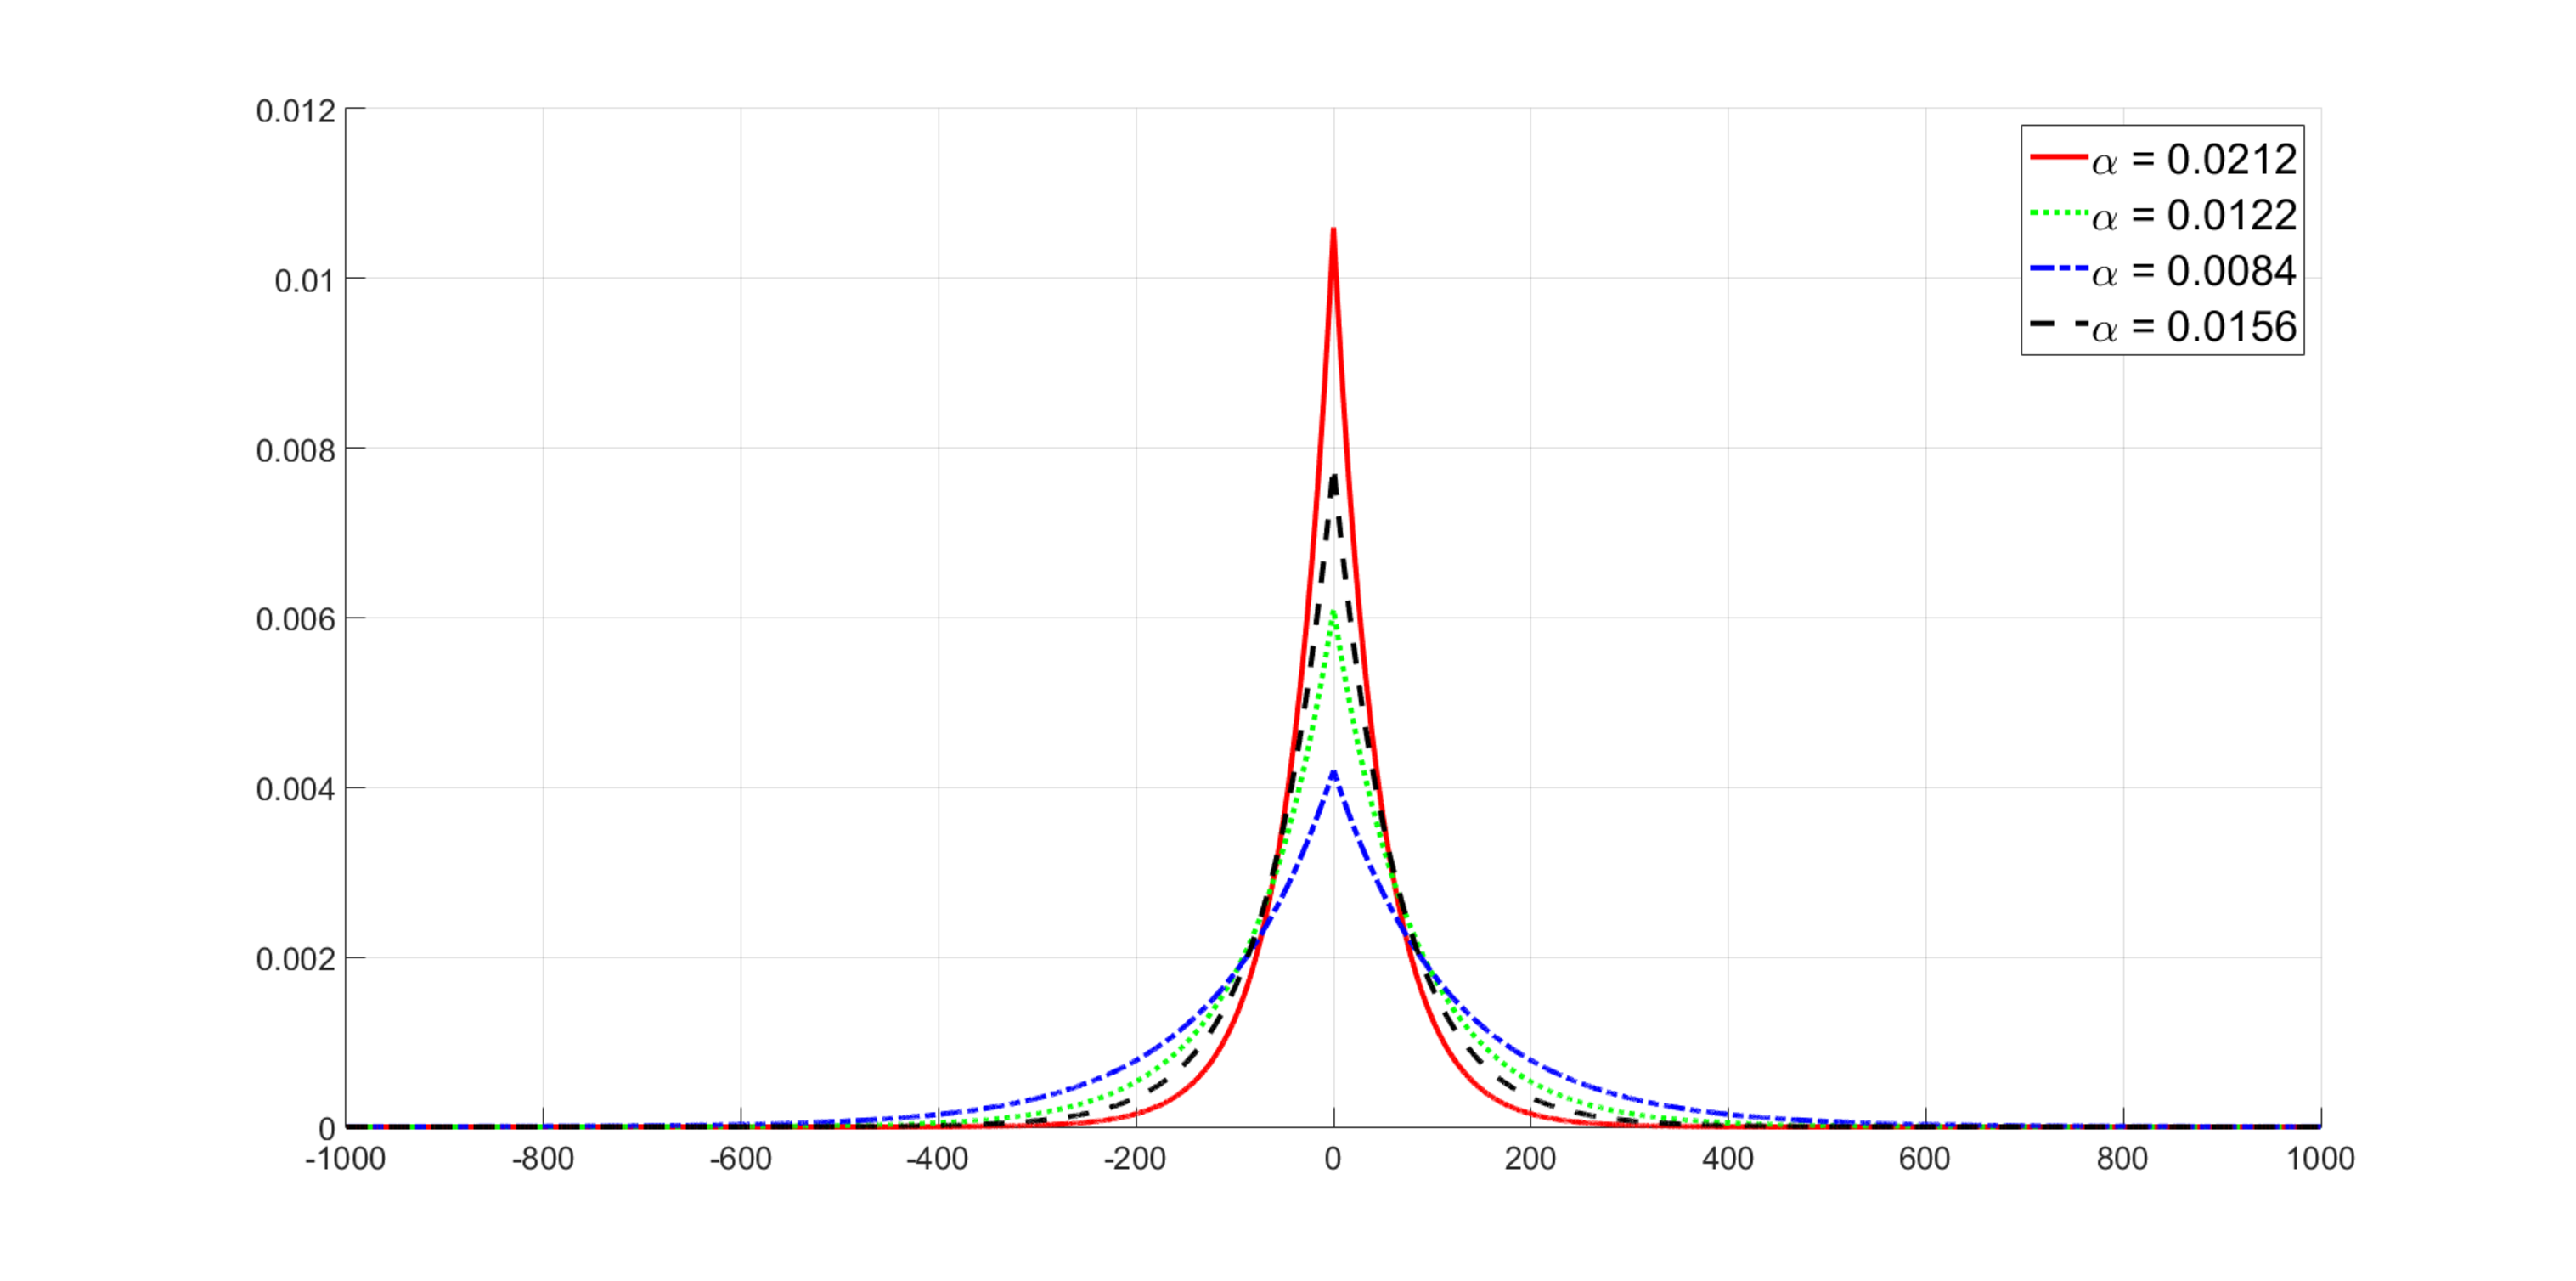
\includegraphics[width=0.9\textwidth]{Chapter3/LaplaceCmp}
    \caption{Функции плотности вероятности для различных значений параметра масштаба.}
    \label{fig:chapCNM:LaplaceCmp}
\end{figure}

\section{Предложенный модифицированный алгоритм оценки параметров ошибок межкадрового предсказания}
\label{chap:CNM:ProposedAlgo}

Основная идея предложенного модифицированного алгоритма оценки параметров ошибок межкадрового предсказания заключается в выполнении разбиения множества $\hat{\mathbf{n}}^{(b)}$ на подмножества и последующей оценке параметров ошибок в каждом подмножестве независимо. Обозначим число подмножеств через $k^{(b)}$. Для выполнения разбиения предлагается использовать подход, основанный на EM-алгоритме~\cite{Bishop:2006:PRM:1162264}. Основная идея EM-алгоритма заключается в следующем. Для каждой случайной величины в выборке вводится скрытая переменная, значение которой может быть вычислено, если известны параметры распределений в смеси. При этом скрытые переменные вводятся таким образом, что, если они известны, можно выполнить пересчет параметров распределений в смеси с использованием принципа максимума правдоподобия.

Приведем описание EM-алгоритма для задачи разбиения множества ошибок на $k^{(b)}$ подмножеств. Будем считать, что смесь имеет вид
\begin{equation}
f(x \vert \mathcal{D}^{(b)}) = \sum\limits_{i=1}^{k^{(b)}} w_i^{(b)} \mathrm{Lap}(x \vert \alpha^{(b)}_{i} ,0).
\label{eq:Mixture}
\end{equation}

Обозначим множество скрытых переменных через $\mathcal{A}^{(b)}$. EM-алгоритм состоит из итеративного повторения двух шагов.
\begin{itemize}
    \item E-шаг. На этом шаге выполняется расчет ожидаемого значения скрытых случайных величин $A_i^{(b)} \in \mathcal{A}^{(b)}$. Обозначим $\Pr[A_i^{(b)} = a \vert N_i^{(b)} = \hat{n}_i^{(b)}]$ через $g_{i,a}$. Тогда на данном шаге выполняются следующие действия:
    \begin{equation}
        \begin{split}
            & \forall a \in \{1,2,\ldots,k^{(b)}\}, \forall i \in \{1,2,\ldots,m\} : 
            \\
            & g_{i,a} = 
            \frac{\Pr\{A_i^{(b)} = a\} \Pr\{N_i^{(b)} = \hat{n}_i^{(b)} \vert A_i^{(b)} = a \}} {\sum\limits_{k=1}^{k^{(b)}} \Pr\{A_i^{(b)} = k\} \Pr\{N_i^{(b)} = \hat{n}_i^{(b)} \vert A_i^{(b)} = k \}} = \frac{w_a^{(b)} \mathrm{p}(\hat{n}_i^{(b)}\vert a)} {\sum\limits_{k=1}^{k^{(b)}} w_k^{(b)} \mathrm{p}(\hat{n}_i^{(b)}\vert k) },
        \end{split}
        \label{eq:EStep}
    \end{equation}
    где $w_a^{(b)} = \Pr\{A_i^{(b)} = a\}$~--~априорное распределение на индексах подмножеств.
    \item M-шаг. На этом шаге выполняется максимизация правдоподобия параметров $\alpha_j^{(b)*}$ и $w_j^{(b)}$ с учетом $\mathcal{A}^{(b)}$:
    \begin{equation}
        \forall a \in \{1,2,\ldots,k^{(b)}\} : w_a^{(b)} = \frac{1}{m} \sum\limits_{i=1}^{m} \mathrm{p}(a \vert \hat{n}_i^{(b)}),
        \label{eq:MStep_w}
    \end{equation}
    \begin{equation}
        \forall a \in \{1,2,\ldots,k^{(b)}\} : \alpha_a^{(b)*} = \arg\max_{\alpha} \sum\limits_{i=1}^{m} g_{i,a} \ln\left(\mathrm{Lap}(\hat{n}_i^{(b)} \vert \alpha, 0)\right).
        \label{eq:MStep_theta}
    \end{equation}
\end{itemize}

Рассмотрим оптимизацию данного выражения. Отметим, что решение оптимизационной данной задачи распадается на $k^{(b)}$ независимых задач. Рассмотрим максимизацию для некоторого индекса $a$.
\begin{equation*}
\begin{split}
\alpha_a^{(b)*} & = \arg\max_{\alpha} \sum\limits_{i=1}^{m} g_{i,a} \ln\left(\mathrm{Lap}(\hat{n}_i^{(b)} \vert \alpha, 0)\right) = \\
& = \arg\max_{\alpha} \sum\limits_{i=1}^{m} g_{i,a} \ln\left( \frac{\alpha}{2}e^{-\alpha \vert \hat{n}_i^{(b)} \vert } \right) = \\
& = \arg\max_{\alpha} \ln(\alpha) \sum\limits_{i=1}^{m} g_{i,a} - \alpha \sum\limits_{i=1}^{m} g_{i,a} \vert \hat{n}_i^{(b)} \vert.
\end{split}
\end{equation*}
Для поиска оптимального значения параметра распределения приравняем производную от получившегося выражения к нулю.
\begin{equation*}
\frac{d}{d\alpha} \left( \ln(\alpha) \sum\limits_{i=1}^{m} g_{i,a} - \alpha \sum\limits_{i=1}^{m} g_{i,a} \vert \hat{n}_i^{(b)} \vert \right) = \frac{1}{\alpha} \sum\limits_{i=1}^{m} g_{i,a} - \sum\limits_{i=1}^{m} g_{i,a} \vert \hat{n}_i^{(b)} \vert = 0.
\end{equation*}
Отсюда получим выражения для $\alpha_a^{(b)*}$:
\begin{equation}
\alpha_a^{(b)*} = \frac{\sum\limits_{i=1}^{m} g_{i,a}}{\sum\limits_{i=1}^{m} g_{i,a} \vert \hat{n}_i^{(b)} \vert}.
\label{eq:AlphaParam}
\end{equation}
Величина~\ref{eq:AlphaParam} рассчитывается на М-шаге EM-алгоритма независимо для каждой из компонент смеси. 

E и M шаги повторяются до тех пор, пока либо значения скрытых переменных $A_i^{(b)}$ не перестанут существенно меняться между итерациями, либо не будет достигнуто максимальное число итераций. Условия сходимости EM-алгоритма рассматриваются в работе~\cite{wu83}. Выходом данной процедуры являются параметры распределений в множестве $\mathcal{D}^{(b)}$, а также веса компонент $w_j$. Для расчета индексов подмножеств предлагается проанализировать вероятности скрытых переменных и выбирать для каждой ошибки то распределение, которое соответствует максимуму апостериорной вероятности события, что ошибка в позиции $i$ получена из распределения с номером~$j$:
\begin{equation}
    \forall i \in \{1,2,\ldots,m\} : a^{(b)}_i = \arg\max_{a \in \{1,2,\ldots,k^{(b)} \} }
    \mathrm{p}(a \vert \hat{n}_i^{(b)}).
\end{equation}

Полученное в результате применения данного алгоритма сопоставление между ошибками и распределениями, задаваемое множеством индексов $\{a^{(b)}_1,a^{(b)}_2,\ldots,a^{(b)}_m\}$ не учитывает тот факт, что ошибки являются зависимыми. Для учета пространственной зависимости предлагается выполнить сглаживающую двумерную фильтрацию данного множества с помощью медианного фильтра, подавив тем самым возможные ошибки сопоставления. В результате, значения $\{a^{(b)}_1,a^{(b)}_2,\ldots,a^{(b)}_m\}$ будут задавать разбиение множества ошибок на подмножества. Далее для оценки параметров ошибок для каждого квантованного спектрального коэффициента предлагается воспользоваться методом из базового алгоритма~\ref{chap:CNM:ReferenceAlgo}. Таким образом, модифицированный алгоритм оценки параметров ошибок межкадрового предсказания для группы спектральных коэффициентов с номером $b$ представляет собой следующую последовательность действий.

\textbf{Входные данные}:
\begin{itemize}
    \item аппроксимация ошибок межкадрового предсказания в спектральной области~--~$\hat{\mathbf{n}}^{(b)}$;
    \item начальное множество параметров распределений в смеси~$\mathcal{L}_{in}^{(b)} = \{ \alpha_1, \alpha_2,\ldots, \alpha_{k^{(b)}}\}$;
    \item начальные значения весов $w_1^{(b)},w_2^{(b)},\ldots,w_{k^{(b)}}^{(b)}$ для компонент смеси;
    \item максимальное число итераций EM-алгоритма~$t_1$;
    \item порог на изменение множества индексов~$t_a$;
    \item начальные значения скрытых переменных $g_{i,a}$, для $i=1,2,\ldots,m$ и $a=1,2,\ldots,k^{(b)}$;
    \item число итераций пространственного сглаживания~$t_2$;
    \item радиус сглаживающего фильтра $r_f$.
\end{itemize}

\textbf{Выходные данные}:
\begin{itemize}
    \item оцененные параметры шума для каждого спектрального коэффициента в группе.
\end{itemize}

\textbf{Алгоритм}.
\begin{enumerate}
    \item\label{algo2:Init} Инициализация:
    \begin{itemize}
        \item $\mathcal{L}^{(b)} = \mathcal{L}_{in}^{(b)}$;
        \item номер итерации EM-алгоритма $t = 1$;
        \item начальная маркировка $a_i=1$, для $i=\overline{1,m}$.
    \end{itemize}
    
    \item\label{algo2:SaveG} Инициализация скрытых переменных:
    \begin{equation*} 
        \forall i \in \{1,2,\ldots,m\}, \forall a \in \{1,2,\ldots,k^{(b)}\}: g_{i,a}^{(0)} = g_{i,a}.
    \end{equation*}
    
    \item\label{algo2:EStep} Расчет ожидаемого значения скрытых случайных величин~$g_{i,a}$ с использованием формулы~(\ref{eq:EStep}).
    
    \item\label{algo2:MStep} Расчет новых весов компонент смеси и параметров распределений с использованием формул~(\ref{eq:MStep_w}) и~(\ref{eq:MStep_theta}).
    
    \item\label{algo2:IterInc} Увеличение номера итерации: $t=t+1$.
    
    \item\label{algo2:EMStopCalc} Расчет критерия остановки предварительной маркировки:
    \begin{equation*}
        Stop = (t > t_1)\text{ или }(\max_{i,a} \vert g_{i,a} - g_{i,a}^{(0)} \vert < t_a).
    \end{equation*}
    
    \item\label{algo2:EMStopAnalyze} Если $Stop$ принимает истинное значение, то переход к шагу~\ref{algo2:MRFRealization}, иначе переход к шагу~\ref{algo2:SaveG}.
    
    \item\label{algo2:MRFRealization} Определение маркировки узлов:
    \begin{equation}
        a_i = \arg\max_{a=\{1,2,\ldots,k^{(b)}\}} g_{i,a}.
    \end{equation}
    
    \item\label{algo2:SpatialFilter} Повторять $t_2$ раз:
    \begin{equation*}
        \begin{split}
            & \forall i \in \{1,2,\ldots,m\}: a_i^{(filt)} = \mathrm{median}(\{a_j\} : d(\mathrm{map}^{-1}(j), \mathrm{map}^{-1}(i)) < r_f ) \\
            & \forall i \in \{1,2,\ldots,m\}: a_i = a_i^{(filt)}
        \end{split},
    \end{equation*}
    где $\mathrm{map}^{-1}(\cdot)$~--~функция, отображающая одномерные индексы в множестве ошибок в двумерные индексы соответствующих блоков на кадре; $\mathrm{median}(\cdot)$~--~функция взятия срединного элемента (медианы) множества.
    
    \item\label{algo2:Mean} Расчет выборочных средних:
    \begin{equation*}
        \forall j \in \{1,2,\ldots,k^{(b)}\} : \mu_j^{(b)} = \frac{1}{\sum\limits_{i=1}^{m} \mathbbm{1}(a_i=j) } \sum_{i=1}^{m} \vert \hat{n}_i^{(b)} \vert \mathbbm{1}(a_i=j),
    \end{equation*}
    где $\mathbbm{1}(\cdot)$~--~индикаторная функция, определенная как
    \begin{equation*}
        \mathbbm{1}(X) = \begin{cases}
            & 1\text{, если $X$ принимает истинное значение} \\
            & 0,\text{ иначе}
        \end{cases}.
    \end{equation*}
    
    \item\label{algo2:Var} Расчет выборочных среднеквадратичных отклонений:
    \begin{equation*}
    \forall j \in \{1,2,\ldots,k^{(b)}\} : \sigma_j^{(b)} = \sqrt{ \frac{1}{\sum\limits_{i=1}^{m} \mathbbm{1}(a_i=j)}   \sum_{i=1}^{m} ( \vert \hat{n}_i^{(b)} \vert - \mu_j^{(b)} )^2 \mathbbm{1}(a_i=j) }
    \end{equation*}
    
    \item Расчет отклонения от выборочного среднего:
    \begin{equation*}
        \forall i \in \{1,2,\ldots,m\} : d_i^{(b)} = (\vert \hat{n}_i^{(b)} \vert - \hat{\mu}_{a_i}^{(b)})^2.
    \end{equation*}
    
    \item\label{algo2:FinalEstimation} Оценка параметров для каждой ошибки:
    \begin{equation*}
        \forall i\in \{1,2,\ldots,m\}:
        \alpha_i^{(b)} = 
        \begin{cases}
            & \frac{\sqrt{2}}{\sigma_{a_i}^{(b)}}\text{, если $ d_i^{(b)}  < (\sigma_j^{(b)})^2$} \\
            & \frac{\sqrt{2}}{d_i^{(b)}}\text{, иначе}
        \end{cases},
    \end{equation*}
    
\end{enumerate}

В завершение описания алгоритма приведем связь предложенного метода с базовым подходом из модели DISCOVER. Пусть для любой группы спектральных коэффициентов начальное множество распределений состоит из одного вероятностного закона, т.~е.~$\mathcal{L}_{in}^{(b)}=\{ \alpha_1 \}$. Тогда на шагах~\ref{algo2:SaveG}-\ref{algo2:MRFRealization} будет осуществляться оценка параметра масштаба $\alpha$ по выборке ошибок $\hat{\mathbf{n}}^{(b)}$. Т.~к. на шаге~\ref{algo2:SpatialFilter} фактически выполняется медианная фильтрация, конфигурация поля распределений меняться не будет. Очевидно, что в таком случае оценка параметров на шагах~\ref{algo2:Mean}-\ref{algo2:FinalEstimation} будет в точности совпадать с оценкой в базовом алгоритме. В том случае, когда начальное множество распределений $\mathcal{L}_{in}^{(b)}$ состоит из $k^{(b)}$ законов, алгоритм будет выполнять разбиение выборки $\hat{\mathbf{n}}^{(b)}$ на максимум $k^{(b)}$ подвыборок, причем по сравнению с базовым алгоритмом оценка интенсивности шума будет снижена для регионов с высоким качеством интерполяции и повышена для регионов с низким качеством интерполяции. Продемонстрируем данное утверждение на примере из подраздела~\ref{chap:CNM:ReferenceAlgo:Troubles}. Напомним, что оценка шума для данного примера имеет следующий вид:
\begin{equation}
    \hat{\mathbf{n}}^{(1)} = 
    \left(
    \begin{matrix}
        2 &  1 &   3 &   5 \\
        0 &  0 &   4 &  83 \\
        7 & 24 & 157 & 208 \\
        1 &  1 &  30 & 132
    \end{matrix}
    \right).
\end{equation}
Матрица коэффициентов масштаба распределения Лапласа, полученная с использованием базового алгоритма:
\begin{equation}
    \left(
    \begin{matrix}
        0.021 & 0.021 & 0.021 & 0.021 \\
        0.021 & 0.021 & 0.021 & 0.021 \\
        0.021 & 0.021 & \textbf{0.012} & \textbf{0.008} \\
        0.021 & 0.021 & 0.021 & \textbf{0.016}
    \end{matrix}
    \right).
\end{equation}
Продемонстрируем работу предложенного алгоритма. Зададим входные параметры:
\begin{itemize}
    \item начальное множество параметров распределений~$\mathcal{L}_{in}^{(b)} = \{0.47, 0.94\}$;
    
    \item начальные значения весов для компонент смеси: $w_1^{(b)}=0.5,w_2^{(b)}=0.5$;
    
    \item максимальное число итераций EM-алгоритма~$t_1=10000$;
    
    \item порог на изменение поля распределений~$t_a=10^{-4}$;
    
    \item начальные значения скрытых переменных $g_{i,a}=0.5$, для $i=1,2,\ldots,16$ и $a=1,2$;
    
    \item число итераций пространственного сглаживания~$t_2=1$;
    
    \item радиус сглаживающего фильтра $r_f=1$.
\end{itemize}

В результате применения EM-алгоритма (шаги 2-7 предложенного алгоритма) через $12$ итераций получим следующее разбиение множества ошибок (шаг 8):
\begin{equation*}
    \left(
    \begin{matrix}
        2  & 2 & 2 & 2 \\
        2  & 2 & 2 & 1 \\
        2  & 1 & 1 & 1 \\
        2  & 2 & 1 & 1
    \end{matrix}
    \right).
\end{equation*}
После медианной фильтрации:
\begin{equation*}
    \left(
    \begin{matrix}
        2  & 2 & 2 & 2 \\
        2  & 2 & 2 & 1 \\
        2  & 2 & 1 & 1 \\
        2  & 2 & 1 & 1
    \end{matrix}
    \right).
\end{equation*}
После применения базового алгоритма независимо в областях, помеченных индексами $1$ и $2$, получаются следующие оценки параметров распределений Лапласа.
\begin{equation*}
    \left(
    \begin{matrix}
        0.206  & 0.206 & 0.206 & 0.206 \\
        0.206  & 0.206 & 0.206 & 0.021 \\
        0.206  & 0.072 & 0.021 & 0.017 \\
        0.206  & 0.206 & 0.015 & 0.021
    \end{matrix}
    \right).
\end{equation*}

Из полученных результатов видно, что по сравнению с базовым, предложенный алгоритм позволяет существенно увеличить разницу в надежности спектральных коэффициентов с малыми и большими оцененными значениями ошибок. Например, коэффициенту со значением $0$, находящемуся на позиции $(2,2)$, базовый алгоритм назначил значение масштаба, равное $0.021$. В то же время, результат преложенного алгоритма для данного коэффициента равен $0.206$.

\section{Описание предложенной аналитической модели виртуального канала}
\label{chap:CNM:ProposedModel}

В начале данного подраздела необходимо отметить, что в настоящее время виртуальный канал рассматривается как некоторое абстрактное понятие. Не существует строгого математического описания модели ошибок в виртуальном канале, что усложняет анализ существующих алгоритмов оценки параметров ошибок межкадрового предсказания и ухудшает понимание специфики и особенностей данной задачи в целом. В связи с этим в данном подразделе вводится в рассмотрение модель искажения промежуточного кадра в процессе его аппроксимации на стороне декодра. В рамках данной модели выполняется формализация понятия виртуального канала и формулируется возможная целевая функция для алгоритмов оценки параметров ошибок межкадрового предсказания.

Рассмотрим расширенный набор допущений о виртуальном канале.

\setcounter{assumptionext}{1}
\begin{assumptionext}[*]
    Виртуальный канал является каналом с аддитивным нестационарным шумом.
    \label{ass:2new}
\end{assumptionext}
Данное допущение обобщает допущение~\ref{ass:2}, позволяя рассматривать не только закон распределения Лапласа. Для определенности будем полагать, что ошибки в виртуальном канале являются случайными величинами, закон распределения каждой из которых принадлежит множеству $\mathcal{D}^{(b)}=\{ D^{(b)}_i(x \vert \boldsymbol{\theta}^{(b)}_i) \}$, $i=\overline{1,k^{(b)}}$, где $D^{(b)}_i(x \vert \boldsymbol{\theta}^{(b)}_i)$ задает вероятностный закон и его параметры для распределения с индексом~$i$. Элементы в множестве $\mathcal{D}^{(b)}$ могут описывать один закон распределения, но в таком случае должны различаться по параметрам. Данное допущение обобщает соответствующее допущение из базового набора, позволяя рассматривать произвольные законы распределений в смеси, а не только распределение Лапласа.

Напомним, что допущение~\ref{ass:2} оперирует с понятием случайной величины $N_i^{(b)}$, реализацией которой является значение ошибки для спектрального коэффициента, находящегося на позиции $i$ в группе спектральных коэффициентов~$b$.

\begin{definition}
    Будем называть множество случайных величин $\mathcal{N}^{(b)}~=~ \left\lbrace N^{(b)}_1, N^{(b)}_2, \ldots, N^{(b)}_m \right\rbrace $ \emph{полем ошибок}.
\end{definition}

\begin{definition}
    Будем называть множество случайных величин $\mathcal{A}^{(b)}~=~ \left\lbrace A^{(b)}_1, A^{(b)}_2, \ldots, A^{(b)}_m \right\rbrace$, где $A^{(b)}_j \in \{1,2,\ldots,k^{(b)}\}$, \emph{полем распределений}.
\end{definition}

Отметим, что для стационарного виртуального канала совместная функция плотности вероятности случайных величин из множества $\mathcal{N}^{(b)}$ задается как
\begin{equation}
f(x \vert \mathcal{D}^{(b)}) = \sum\limits_{i=1}^{k^{(b)}} w_i^{(b)} D_i^{(b)}(x \vert \boldsymbol{\theta}_i^{(b)}).
\label{eq:GeneralMM}
\end{equation}

Для сокращения обозначений далее не будем указывать формальный параметр $x$ при написании закона распределения.

В процессе моделирования виртуального канала каждой случайной величине из $\mathcal{N}^{(b)}$ должно быть сопоставлено распределение из $\mathcal{D}^{(b)}$. Будем обозначать событие, что $N_i^{(b)}$ имеет закон распределения $D_j^{(b)}(\boldsymbol{\theta}_j^{(b)})$, как $N_i^{(b)} \sim D_j^{(b)}(\boldsymbol{\theta}_j^{(b)})$. Событие, заключающееся в сопоставлении законов распределений из $\mathcal{D}^{(b)}$ со случайными величинами из $\mathcal{N}^{(b)}$, можно рассматривать как реализацию случайного поля $\mathcal{A}^{(b)}$. Нестационарность шума в виртуальном канале означает, что
\begin{equation*}
\Pr \left[ \bigcap\limits_{i=1}^{m} A_i^{(b)}=a_i \right] \neq 
\prod\limits_{i=1}^{m} \Pr \{ A_i^{(b)}=a_i ] \}
\end{equation*}

\begin{assumptionext}
    Поле распределений является Марковским случайным полем.
\label{ass:3new}
\end{assumptionext}

\begin{definition}
    Марковское случайное поле, или сеть Маркова,~--~это случайное поле, обладающее Марковским свойством, описанным неориентированным графом.
\end{definition}

Допущения~\ref{ass:2new} и~\ref{ass:3new} позволяют рассматривать процесс появления шума с точки зрения вероятностной порождающей модели (PGM, Probabilistic Generative Model). На качественном уровне появление шума в данной модели можно пояснить следующим образом. Следующие шаги выполняются для каждого спектрального коэффициента.
\begin{enumerate}
  \item С помощью некоторой процедуры выбирается распределение из $\mathcal{D}^{(b)}$ так, чтобы учитывать пространственную зависимость законов распределений ошибок спектральных коэффициентов соседних блоков;
  \item В соответствии с выбранным законом генерируется случайная величина, соответствующая ошибке в данном спектральном коэффициенте.
\end{enumerate}

Подобная модель позволяет свести задачу оценки параметров ошибок межкадрового предсказания к согласованному сопоставлению ошибок и распределений из~$\mathcal{D}^{(b)}$.

Напомним, что для того, чтобы задать МСП необходимо определить множество случайных величин (узлы графа) и вероятностные зависимости (дуги графа) между ними~(приложение~\ref{AppA}). 

Зададим МСП над множеством случайных величин $\mathcal{A}^{(b)}$. Для этого введем в рассмотрение регулярную прямоугольную решетку узлов $\mathcal{S}^{(b)}$ как:
\begin{equation*}
\mathcal{S}^{(b)} = \left\lbrace (i,j)^T \vert i=\{1,2,\ldots,h_{b}\}, j=\{1,2,\ldots,w_{b}\} \right\rbrace,
\end{equation*}
где $w_{b}=\frac{w}{4}$ и $h_{b}=\frac{h}{4}$, $w$ и $h$ ширина и высота кадра $\mathbf{F}_a$ соответственно. Делитель $4$ задается размером блока в  дискретном косинусном преобразовании, т.~е. $w_{b}$ и $h_{b}$ определяют число спектральных коэффициентов в одной группе:
\begin{equation*}
m=w_{b}\times h_{b}.
\end{equation*}
Здесь и далее будем использовать понятия <<узел>> и <<позиция узла>> как синонимы. Следует отметить, что узлы в множестве $\mathcal{S}^{(b)}$ задают на плоскости прямоугольную регулярную решетку, координаты в которой можно рассматривать как индексы блоков при дискретном косинусном преобразовании. Отметим также, что так как число спектральных коэффициентов не меняется между группами, координаты в решетке не привязаны к конкретному номеру $b$. Следуя данному соглашению, сопоставим элементы множества $\mathcal{A}^{(b)}$ c узлами решетки, для определенности предполагая, что спектральные коэффициенты в группе формировались с помощью обхода блоков по столбцам:
\begin{equation}
\begin{split}
& A_1^{(b)} \leftrightarrow (1,1)^T \\
& A_2^{(b)} \leftrightarrow (2,1)^T \\
& \cdots \\
& A_{h_{b}}^{(b)} \leftrightarrow (h_{b},1)^T \\
& A_{h_{b}+1}^{(b)} \leftrightarrow (1,2)^T \\
& \cdots \\
& A_m^{(b)} \leftrightarrow (h_{b},w_{b})^T
\end{split}.
\label{eq:MappingGridToVec}
\end{equation}

Отметим, что сопоставление~\ref{eq:MappingGridToVec} задает взаимно однозначное отображение множества одномерных индексов случайных величин из~$\mathcal{A}$ на множество узлов двумерной решетки. Для приведенного порядка обхода данное отображение можно определить как следующую функцию:
\begin{equation}
\mathrm{map}(i,j) = i + (j-1)h_b.
\label{eq:MappingGridToVecFunction}
\end{equation}

Далее определим свойство Марковости для случайного поля~$\mathcal{A}$. Для этого зададим отношение соседства над узлами из $\mathcal{S}^{(b)}$:
\begin{equation*}
\mathcal{R}^{(b)} = \{ \mathcal{R}_{i,j}^{(b)} \vert \forall (i,j)^T \in \mathcal{S}^{(b)} \},
\end{equation*}
где $\mathcal{R}_{i,j}^{(b)}$~--~множество соседей узла $(i,j)^T$. На регулярной решетке это множество можно задать следующим образом:
\begin{equation*}
\mathcal{R}_{i,j}^{(b)} = \{ (i',j')^T \in \mathcal{S}^{(b)} \vert 0 < \mathrm{d}((i,j)^T,(i',j')^T) \leq r \},
\end{equation*}
где $r$~--~параметр, определяющий количество соседей; функция $\mathrm{d}((i,j)^T,(i',j')^T)$ задает Евклидово расстояние в двумерном пространстве:
\begin{equation*}
\mathrm{d}((i,j)^T,(i',j')^T) = \sqrt{(i-i')^2+(j-j')^2}.
\end{equation*}
Таким образом, соседями узла $(i,j)^T$ являются те узлы, которые находятся от него на расстоянии не больше, чем $r$. Для Марковского случайного поля это означает, что
\begin{equation}
    A_{i,j} \CI \mathcal{A}\setminus\mathcal{R}_{i,j}^{(b)} \mid \mathcal{R}_{i,j}^{(b)}.
\end{equation}

Множество $\mathcal{R}^{(b)}$ определяет вероятностные связи между случайными величинами из $\mathcal{A}^{(b)}$. На графической вероятностной модели для случайного поля эта зависимость выражается в наличии дуг между вершиной $(i,j)^T$ и её соседями из $\mathcal{R}_{i,j}$. Таким образом упорядоченная пара множеств $\left(\mathcal{S}^{(b)}, \mathcal{R}^{(b)}\right)$ задает граф $\mathcal{G}^{(b)}$, соответствующий МСП над множеством случайных величин~$\mathcal{A}^{(b)}$. 

Рассмотрим связь описанного МСП с полученной на стороне декодера аппроксимацией шума. Конкретная реализация МСП задает разбиение множества случайных величин  $\mathcal{N}^{(b)}$ на несколько подмножеств, причем в каждом подмножестве случайные величины имеют один закон распределения. В таком случае шум представляет собой реализацию поля $\mathcal{N}^{(b)}$ с учетом скрытых случайных величин $\mathcal{A}^{(b)}$. Таким образом, модель шума описывается скрытым Марковским случайным полем (СМСП), где наблюдаемым случайными величинами являются $N_1^{(b)}$, $N_2^{(b)}$,\ldots,$N_m^{(b)}$, а скрытыми~--~$A_1^{(b)}$, $A_2^{(b)}$,\ldots,$sA_m^{(b)}$. Пример вероятностной графической модели для $r=\sqrt{2}$ приведен на рисунке~\ref{fig:chap3:HMRF}.

\begin{figure}[htbp]
  \centering
  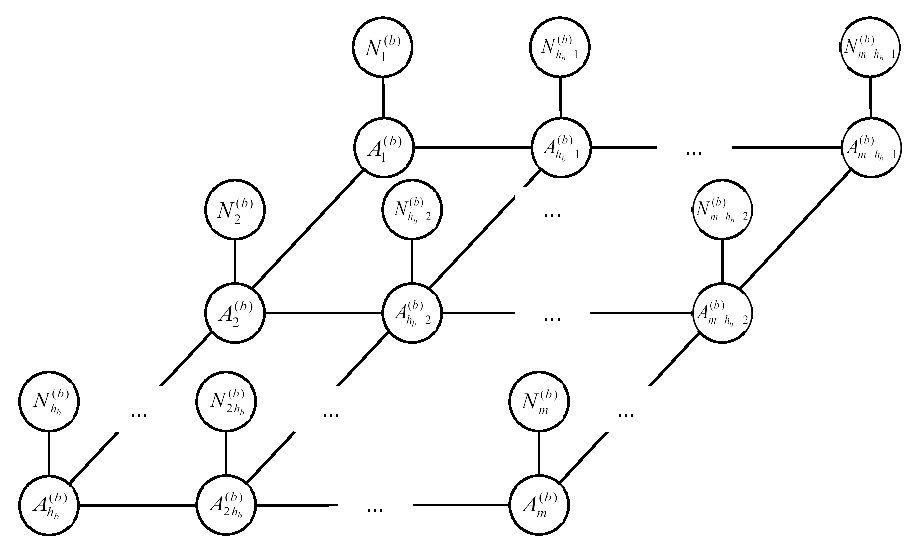
\includegraphics[width=0.9\textwidth]{Chapter3/HMRF}
  \caption{Пример вероятностной графической модели для скрытого Марковского случайного поля.}
  \label{fig:chap3:HMRF}
\end{figure}

С учетом приведенной модели задачу моделирования виртуального канала для группы спектральных коэффициентов с номером $b$ можно свести к решению следующей оптимизационной задачи:
\begin{equation}
\begin{split}
\mathbf{a}^{(b)*}
& = \arg\max_{\mathbf{a} \in \{1,2,\ldots,k^{(b)}\}^m} \mathrm{p}(\mathbf{a} \vert \hat{\mathbf{n}}^{(b)} ) = \\
& = \arg\max_{\mathbf{a} \in \{1,2,\ldots,k^{(b)}\}^m}
\frac{\mathrm{p}(\hat{\mathbf{n}}^{(b)} \vert \mathbf{a})\mathrm{p}(\mathbf{a})}{\mathrm{p}(\hat{\mathbf{n}}^{(b)})} = \\
& = \arg\max_{\mathbf{a} \in \{1,2,\ldots,k^{(b)}\}^m}
\mathrm{p}(\hat{\mathbf{n}}^{(b)} \vert \mathbf{a})\mathrm{p}(\mathbf{a})
\end{split}.
\label{eq:MRFOptimization}
\end{equation}
где
\begin{equation}
\mathrm{p}(\hat{\mathbf{n}}^{(b)} \vert \mathbf{a}) = \Pr \left\lbrace \bigcap\limits_{i=1}^{m} N_i^{(b)} = \hat{n}_i^{(b)} \bigg\vert \bigcap\limits_{i=1}^{m} A_i^{(b)} = a_i^{(b)} \right\rbrace,
\label{eq:MRFModelLikelihood}
\end{equation}
\begin{equation}
\mathrm{p}(\mathbf{a}) = \Pr \left\lbrace \bigcap\limits_{i=1}^{m} A_i^{(b)} = a_i^{(b)} \right\rbrace.
\end{equation}

Т.~е. $\mathrm{p}(\hat{\mathbf{n}}^{(b)} \vert \mathbf{a})$ является правдоподобием поля распределений для аппроксимации шума $\hat{\mathbf{n}}^{(b)}$, а $\mathrm{p}(\mathbf{a})$ описывает априорное распределение вероятностей над множеством реализаций поля распределений.

Учитывая, что случайные величины $N_i^{(b)}$ независимы при известной реализации поля распределений $\mathcal{A}^{(b)}$, а также воспользовавшись свойствами условной независимости случайных величин в поле распределений, упростим выражение~(\ref{eq:MRFModelLikelihood}):
\begin{equation}
\mathrm{p}(\hat{\mathbf{n}}^{(b)} \vert \mathbf{a}) = \prod\limits_{i=1}^{m} \mathrm{p} (\hat{n}_i^{(b)} \vert \mathbf{a}) = \prod\limits_{i=1}^{m}\mathrm{p} (\hat{n}_i^{(b)} \vert a_i).
\end{equation}

Рассмотрим теперь выражение для априорного распределения вероятностей над множеством реализаций поля распределений. Согласно теореме Хаммерсли-Клиффорда~\cite{Li:2009:MRF:1529944}, случайное поле $\mathcal{A}^{(b)}$ является полем Гиббса, и, следовательно, совместная плотность случайных величин из $\mathcal{A}^{(b)}$ может быть факторизована на кликах графа $\mathcal{G}^{(b)}$:
\begin{equation}
\mathrm{p}(\mathbf{a}) = \frac{1}{z} \exp\left(-\frac{1}{t}U(\mathbf{a})\right),
\end{equation}
где $t$~--~параметр распределения Гиббса; $z$~--~коэффициент нормировки, определяемый как
\begin{equation}
z = \sum_{\mathbf{a} \in \{1,2,...,k^{(b)}\}^m} \exp\left(-\frac{1}{t}U(\mathbf{a})\right);
\end{equation}
$U(\mathbf{a})$~--~сумма потенциальных функций на кликах графа $\mathcal{G}^{(b)}$. Обозначим множество клик $\mathcal{G}^{(b)}$ через $\mathcal{C}$, тогда
\begin{equation}
U(\mathbf{a}) = \sum_{c \in \mathcal{C}} \psi_{c}(\mathbf{a}),
\end{equation}
где $\psi_{c}(\cdot)$~--~потенциалы клик.

Учитывая вышеприведенные соотношения, перепишем оптимизационную задачу~(\ref{eq:MRFOptimization}):
\begin{equation}
\begin{split}
\mathbf{a}^{(b)*} & = \arg\max_{\mathbf{a} \in \{1,2,\ldots,k^{(b)}\}^m} \mathrm{p}(\hat{\mathbf{n}}^{(b)} \vert \mathbf{a}) \mathrm{p}(\mathbf{a}) \\
& = \arg\max_{\mathbf{a} \in \{1,2,\ldots,k^{(b)}\}^m} \prod\limits_{i=1}^{m}\mathrm{p} (\hat{n}_i^{(b)} \vert a_i) \frac{1}{z} \exp\left(-\frac{1}{t}\sum_{c \in \mathcal{C}} \psi_{c}(\mathbf{a})\right) \\ 
& = \arg\max_{\mathbf{a} \in \{1,2,\ldots,k^{(b)}\}^m} \prod\limits_{i=1}^{m} \mathrm{p} (\hat{n}_i^{(b)} \vert a_i) \exp\left(-\frac{1}{t}\sum_{c \in \mathcal{C}} \psi_{c}(\mathbf{a})\right)
\end{split}.
\label{eq:MRFOptimizationGeneral}
\end{equation}

Выражение~(\ref{eq:MRFOptimizationGeneral}) является общей целевой функцией при решении задачи моделирования виртуального канала. Отметим, что в данном выражении в явном виде не задаются ни вероятности, связывающие наблюдаемые ошибки $\hat{n}_i^{(b)}$ с индексами распределений $a_i$, из которых они получены, ни конкретный вид функций $\psi_{c}(\mathbf{a})$.

Рассмотрим один частный случай оптимизации~(\ref{eq:MRFOptimizationGeneral}) в предположении, что правдоподобие поля $\mathcal{A}^{(b)}$ задается параметрическим семейством экспоненциальных распределений, т.~е.
\begin{equation*}
\forall j \in \{1,2,...,k^{(b)}\}: D_j^{(b)} (x \vert \boldsymbol{\theta}_j^{(b)}) = \zeta(\boldsymbol{\theta}_j^{(b)}) \exp\left( -\phi_j(x, \boldsymbol{\theta}_j^{(b)}) \right),
\label{eq:ExponentialFamily}
\end{equation*}
где $\zeta(\boldsymbol{\theta}_j^{(b)})$~--~некоторый коэффициент, зависящий от параметров распределения; $\phi_i(\cdot,\cdot)$~--~некоторая функция, обратно пропорциональная правдоподобию распределения из~$\mathcal{D}^{(b)}$. Напомним, что к семейству экспоненциальных распределений относятся все дискретные, а также многие непрерывные распределения (например, распределения Гаусса, Лапласа, Дирихле, Бэта и т.~д.).

Используя выражение~(\ref{eq:ExponentialFamily}), оптимизационную задачу ~(\ref{eq:MRFOptimizationGeneral}) можно упростить следующим образом:
\begin{equation}
\begin{split}
& \mathbf{a}^{(b)*} = \arg\max_{\mathbf{a} \in \{1,2,\ldots,k^{(b)}\}^m}
\prod\limits_{i=1}^{m} \mathrm{p} (\hat{n}_i^{(b)} \vert a_i) \exp\left(-\frac{1}{t}\sum_{c \in \mathcal{C}} \psi_{c}(\mathbf{a})\right) = \\
& = \arg\max_{\mathbf{a} \in \{1,2,\ldots,k^{(b)}\}^m}
\left[ \prod\limits_{i=1}^{m} \zeta(\boldsymbol{\theta}_{a_i}^{(b)}) \exp\left( -\phi_i(\hat{n}_i^{(b)}, \boldsymbol{\theta}_{a_i}^{(b)}) \right)\right] \exp\left(-\frac{1}{t}\sum\limits_{c \in \mathcal{C}} \psi_{c}(\mathbf{a})\right) = \\
& = \arg\max_{\mathbf{a} \in \{1,2,\ldots,k^{(b)}\}^m}
\left[\prod\limits_{i=1}^{m} \zeta(\boldsymbol{\theta}_{a_i}^{(b)})\right]
\exp\left( -\sum\limits_{i=1}^{m}\phi_i(\hat{n}_i^{(b)}, \boldsymbol{\theta}_{a_i}^{(b)}) -\frac{1}{t} \sum\limits_{c \in \mathcal{C}} \psi_{c}(\mathbf{a}) \right) = \\
& = \arg\max_{\mathbf{a} \in \{1,2,\ldots,k^{(b)}\}^m}
\sum\limits_{i=1}^{m} \ln \zeta(\boldsymbol{\theta}_{a_i}^{(b)}) - \sum\limits_{i=1}^{m}\phi_i(\hat{n}_i^{(b)}, \boldsymbol{\theta}_{a_i}^{(b)}) -\frac{1}{t} \sum\limits_{c \in \mathcal{C}} \psi_{c}(\mathbf{a}) = \\
& = \arg\min_{\mathbf{a} \in \{1,2,\ldots,k^{(b)}\}^m}
\sum\limits_{i=1}^{m} \left(\phi_i(\hat{n}_i^{(b)}, \boldsymbol{\theta}_{a_i}^{(b)}) - \ln\zeta(\boldsymbol{\theta}_{a_i}^{(b)})\right) + \frac{1}{t} \sum\limits_{c \in \mathcal{C}} \psi_{c}(\mathbf{a}).
\end{split}
\label{eq:MRFOptimizationExponential}
\end{equation}

Обозначим $\left[\phi_i(\hat{n}_i^{(b)}, \boldsymbol{\theta}_{a_i}^{(b)}) - \ln\zeta(\boldsymbol{\theta}_{a_i}^{(b)})\right]$ через $\varphi_i(\hat{n}_i^{(b)}, \boldsymbol{\theta}_{a_i}^{(b)})$ и положим $t=1$, тогда
\begin{equation}
\mathbf{a}^{(b)*} = \arg\min_{\mathbf{a} \in \{1,2,\ldots,k^{(b)}\}^m}
\sum\limits_{i=1}^{m} \varphi_i(\hat{n}_i^{(b)}, \boldsymbol{\theta}_{a_i}^{(b)}) + \sum\limits_{c \in \mathcal{C}} \psi_{c}(\mathbf{a}).
\label{eq:MRFOptimizationExp}
\end{equation}

Рассмотрим получившееся выражение. Для определенности зададим $r=\sqrt{2}$, т.~е. множество соседей для каждого узла включает только те узлы, которые находятся на расстоянии не больше $\sqrt{2}$ от него. Данная конфигурация соответствует графу $\mathcal{G}^{(b)}$ с кликами, состоящими либо из одной вершины, либо из пары вершин (рисунок~\ref{fig:chap3:HMRF}). Тогда выражение~\ref{eq:MRFOptimizationExp} можно переписать следующим образом:
\begin{equation}
\mathbf{a}^{(b)*} = \arg\min_{\mathbf{a} \in \{1,2,\ldots,k^{(b)}\}^m}
\left[ E_{data}(\mathbf{a},\mathbf{\hat{n}}^{(b)}) + E_{smooth}(\mathbf{a}) + E_{label}(\mathbf{a}) \right],
\label{eq:PairwiseMRFOptimizationExp}
\end{equation}
где
\begin{equation*}
E_{data}(\mathbf{a},\mathbf{\hat{n}}^{(b)}) = \sum\limits_{i=1}^{m} \varphi_i(\hat{n}_i^{(b)}, \boldsymbol{\theta}_{a_i}^{(b)}),
\end{equation*}
\begin{equation*}
E_{smooth}(\mathbf{a}) = \sum\limits_{i = 1}^{m} \sum\limits_{j \in \mathcal{R}_i} \psi_{i,j}(a_i,a_j),
\end{equation*}
\begin{equation*}
E_{label}(\mathbf{a}) = \sum\limits_{i = 1}^{m} \psi_{i}(a_i).
\end{equation*}

Таким образом, в процессе минимизации выражения~\ref{eq:PairwiseMRFOptimizationExp} осуществляется поиск такой конфигурации поля распределений, которая одновременно:
\begin{itemize}
  \item уменьшает невязку наблюдаемых случайных величин $\hat{n}_i^{(b)}$ с сопоставленными им законами распределений (минимизация слагаемого $E_{data}$);
  \item учитывает пространственную зависимость распределений, уменьшая рассогласование между метками соседних коэффициентов (минимизация слагаемого $E_{smooth}$);
  \item позволяет задавать априорную информацию о маркерах распределений (минимизация слагаемого $E_{label}$).
\end{itemize}

Следует отметить, что данная теоретическая модель обладает рядом особенностей.
\begin{itemize}
    \item В общем случае для произвольных функций $\varphi_i(\cdot)$, $\psi_i(\cdot)$ и $\psi_{i,j}(\cdot,\cdot)$,  минимизация~(\ref{eq:PairwiseMRFOptimizationExp}) является NP-полной задачей и требует перебора $(k^{(b)})^m$ различных реализаций поля распределений для поиска глобального минимума. Однако, для некоторых классов функций потенциалов, в частности, когда данные функции являются метриками или полу-метриками, существуют алгоритмы, которые позволяют находить локальный минимум выражения~(\ref{eq:PairwiseMRFOptimizationExp}).
    \item Параметризация данной модели, а именно задача, связанная с определением вида функций  $\varphi_i(\cdot)$, $\psi_i(\cdot)$ и $\psi_{i,j}(\cdot,\cdot)$, является в настоящее время открытой. В общем случае, не существует алгоритма подбора функций, описывающих зависимости между случайными величинами в Марковском случайном поле. Более того, данная задача является задачей без ограничений в бесконечномерном пространстве функций, что исключает возможность её решения без наложения ограничений, например, на семейство функций. Следует отметить, что при наличии ограничений такого рода, задача может быть решена, например, с использованием алгоритмов обучения графических моделей~\cite{Koller}.
\end{itemize}

В завершение описания модели приведем значения целевой функции, которые получаются при использовании базового и модифицированного алгоритма. Расчет будем проводить для примера, разобранного в подразделах~\ref{chap:CNM:ReferenceAlgo:Troubles} и~\ref{chap:CNM:ProposedModel}. Для определенности будем полагать, что Марковское случайное поле описывается четырехсвязным графом (рисунок~\ref{fig:chap3:HMRF}). Совместную плотность для <<смежных>> случайных величин зададим как экспоненциальное распределение от разности между параметрами масштаба, рассчитанными для распределения Лапласа в позициях соответствующих коэффициентов:
\begin{equation*}
p(a_i,a_j) = \lambda e^{(-\lambda \vert \alpha_{a_i} - \alpha_{a_j} \vert)}, \forall i,j : i \neq j\text{ и }\vert i^2-j^2 \vert <\sqrt{2}.
\end{equation*}
Зададим значение коэффициента $\lambda=1$.
Значения оцененных ошибок межкадрового предсказания:
\begin{equation*}
\hat{\mathbf{n}}^{(1)} = 
\left(
\begin{matrix}
2 &  1 &   3 &   5 \\
0 &  0 &   4 &  83 \\
7 & 24 & 157 & 208 \\
1 &  1 &  30 & 132
\end{matrix}
\right).
\end{equation*}
Результат базового алгоритма:
\begin{equation*}
\left(
\begin{matrix}
0.021 & 0.021 & 0.021 & 0.021 \\
0.021 & 0.021 & 0.021 & 0.021 \\
0.021 & 0.021 & 0.012 & 0.008 \\
0.021 & 0.021 & 0.021 & 0.016
\end{matrix}
\right).
\end{equation*}
Результат модифицированного алгоритма:
\begin{equation*}
\left(
\begin{matrix}
0.206  & 0.206 & 0.206 & 0.206 \\
0.206  & 0.206 & 0.206 & 0.021 \\
0.206  & 0.072 & 0.021 & 0.017 \\
0.206  & 0.206 & 0.015 & 0.021
\end{matrix}
\right).
\end{equation*}
Значение логарифма от целевой функции для базового алгоритма составляет $-83.85$, для модифицированного алгоритма~--~$-70.3$, т.~е. с точки зрения рассмотренной модели модифицированный алгоритм выполняет более вероятное назначение распределений оцененным ошибкам межкадрового предсказания.

\section{Выводы}

В данном разделе были рассмотрены вопросы, связанные с оценкой параметров ошибок в виртуальном канале в рамках систем распределенного кодирования видеоданных. Основные результаты раздела можно сформулировать следующим образом:
\begin{itemize}
    \item проанализирован алгоритм оценки параметров ошибок межкадрового предсказания, используемый в базовой модели распределенного кодирования на основе проекта DISCOVER, выделены его основные особенности и недостатки;
    \item предложена модификация алгоритма оценки параметров ошибок межкадрового предсказания, учитывающая свойство группировки ошибок с большой амплитудой;
    \item введен новый, расширенный, набор допущений о виртуальном канале;
    \item предложена аналитическая модель виртуального канала, основанная на моделировании ошибок межкадрового предсказания как случайного процесса, описываемого скрытым Марковским случайным полем.
\end{itemize}

Вопросы, связанные со сравнительной оценкой модифицированного и базового алгоритмов, рассматриваются в разделе~\ref{chap:ExpResults} данной диссертационной работы.